\chapter{Related Work}
The related work referenced here influenced the decisions for the kind of charitable giving implemented, the general structure of the system, and design decisions regarding the roles of users in the system. Smart Sponsor will be based both on psychological results/studies and the Smart Money concept. Although many of these paper refer to traditional charity systems, the "Charity Aid Foundation" groups sponsoring into the same category as traditional charities \cite{giving19}\cite{giving20}\cite{giving21}. 
\section*{Psychology behind Giving}
Bekkers et al.\cite{psych} analyzed multiple studies and other papers and compiled eight primary reasons for giving and donating. These eight reasons and to what extent Smart Sponsor addresses them are compiled in Figure 2.1. There are two reasons for an aspect to not be in focus for Smart Sponsor. Either the system does not try to address these aspects or the use of a blockchain does not make a difference.
\begin{figure}[H]
    \centering
    \begin{center}
    \begin{tabular}{ | m{12em} | m{3cm}|} 
    \hline
    Efficacy \newline Values  & Focus  \\ 
    \hline
    Reputation \newline Cost and Benefits & Partial  Focus\\ 
    \hline
    Awareness of Need \newline Solicitation \newline Altruism \newline Psychological Benefits & No Focus \\ 
    \hline
    \end{tabular}
    \end{center}
    \caption{The eight reasons behind donating as by Bekkers et al\cite{psych} and how much Smart Sponsor attempts to address them}
    \label{fig:my_label}
\end{figure}

 The two factors Smart Sponsor attempts to address the most are "Efficacy" and "Values". "Efficacy" describes the donors' perception their donation is having a positive impact on society and whether the money reaches the people the donor intends to. As Smart Sponsor would not allow money to be used for purposes not intended the efficacy should increase, consequently furthering willingness to donate. Smart Sponsor addresses "Values" twofold. Firstly, as the recipient has to fulfill qualities, values about the person e.g. "Is from my hometown" can be enforced. Secondly, it can also be ascertained that the stores, the recipient spends the money at, fulfill values e.g. "Fair Trade".\\
 The "Reputation" factor is partially addressed as it is possible to prove one has donated a certain amount to a certain organization. Still, this part is not in the foreground and is merely a byproduct. "Cost and Benefits" is the factor regarding how much money one should ask for when soliciting to have the best outcome. Smart Sponsor allows the donors to donate variable amounts and furthermore, there are no costs associated with the money transfer which is a benefit many blockchain applications offer \cite{disberse}\cite{alice}.\\
 The "Altruism" and "Psychological Benefits" factors do not vary depending on the form the donation takes, so they are not in Focus. Similarly "Awareness of Need" and "Solicitation" are not in Focus as Smart Sponsor instead attempts to increase trust in charity organizations.
\section*{Programmable Donations}
Elsden et al.\cite{progDon} held an interview study focusing on "Escrow" (fiduciary) based programmable donations. An escrow is a third party holding on to the funds of a transaction and releasing them once a predefined condition is met. These donations would then deal with the "first mile" \cite{progDon}, the problem of transferring money from individual donors to charity organizations. The participants were asked to fill in cards containing 3 blank spaces, detailing how often to spend an amount on what condition. Examples the participants gave were  "Donate a certain amount when an earthquake occurs, as certified by a news site." or "Donate the price of a bus ticket, every time I take the car to work, verified by me."\cite{progDon}.
The donations broadly fell into the categories presented by these examples. The first is classical donations and the second is more along the lines of self-imposed taxes. Elsden et al. conjectured the second case to be a possible direction for the future role of charities but Smart Sponsor is more concerned with the traditional donation-based systems.
\\
After setting up these conditions the participants were interviewed regarding their impressions and their willingness to use an escrow-based donation system. Some participants felt uneasy using such a system. People usually donate money because they want to have a positive impact on society and the money instead being locked in an escrow caused dissonance \cite{progDon}. Furthermore, the prospect of money that was not spent by the end of the time limit given to the escrow, being returned to the donor felt unpleasant. Usually, people feel they have done the good deed and parted with their money as they donated it and they rather not want to get it returned \cite{progDon}. Setting conditions was also another point of concern. Both the money donated and the trigger for a donation to occur would have to be thought out carefully which takes time and energy. Many people want to experience the pleasant feeling of having helped someone and putting this much consideration into how and when to help someone felt too calculating and mentally draining \cite{progDon}. \\
Therefore Smart Sponsor will try to make the donation process not exhausting. Especially the possibility of no one fulfilling the donation conditions needs to be addressed as in this case the money would be returned to the donor at some point. Too many complexities might be counterproductive here.
\section*{HCI Research on Philanthropic IT}
Harmon et al.\cite{philit} talk about the importance of adopting new technologies into systems for charities. At the same time they warn about the propensity of the IT sector to design new systems for donations systems that in theory could help them but in practice cause stress and friction.\\
As Smart Sponsor is not so much traditional donating, but more akin to a scholarship, charity organizations are taken out of the equation. In this case, the increased workload falls upon the recipient who has to prove they fulfill the conditions. Smart Sponsor will therefore not allow too complicated conditions to ensure the effort of proving one's credentials doesn't outweigh the benefit of the donation.\\
It is also very important to treat the privacy of a recipient with the out-most care. Therefore it should not be possible to reverse engineer information from the certificates the third-party verifier holds. At the same time, it has to be possible for systems like Smart Sponsor to access these certificates to ascertain a recipient's validity.
\section*{Current Blockchain-based Applications}
Currently, there seem to be broadly two different categories of blockchain-based donation applications:\\
One group are donation applications that gather cryptocurrencies and use these to support projects \cite{bitgive}\cite{binance}\cite{giveBlock}\cite{engiven}. These applications vary in the recipient, be it a traditional charity organization supporting projects or individuals who can apply for help independently. This kind of service offers both the transparency donors desire and at the same time, it also allows for a reduction in transaction fees that might be incurred by supporting organizations in foreign countries \cite{engiven}. On the other hand, cryptocurrencies are quite volatile and also still a young technology \cite{willing}. This volatility is an aspect to consider when looking to support a project where stability is also a very important factor. Furthermore, the public perception of cryptocurrencies is not very positive. This is due to the amount of illicit activity around cryptocurrencies, but also because cryptocurrencies as a concept are still very new \cite{willing}. In 2018, 29\% of Europeans would not even consider investing in cryptocurrencies and therefore this project will be using tokenized fiat currencies instead \cite{willing}.\\
The other category of service is focused on the "Last mile" \cite{progDon}. These services focus on the charity organizations showing results. After a certain amount of currency (crypto or fiat) is pledged to a goal, the charity organization starts working on the project until they hit a predetermined first milestone. At this point, the donors are notified of the progress and get to decide if the organization has fulfilled their intentions and should receive the funds for the next milestone \cite{alice}\cite{promisegive}.\\
These systems satisfy the need for efficacy in the charity. At the same time, this concept can run into the problems that have been described by Elsden et al.\cite{progDon}. The possible release of funds back to donors is an aspect that should be considered. Furthermore, this system does require more effort on the donor's side if they want to use the system as it is intended. Spending the time to research if the money was used to one's intentions takes of course time and energy, but it also can give the donor a feeling of moving himself too much into the foreground \cite{progDon}. Therefore Smart Sponsor should be seen as a complementing alternative for donors who want to donate in the classical way but have an increased level of control over the use of their money.
\section*{Smart Money/Currency}
It is important to differentiate between the two uses of the term "Smart Money/Currency". The first is just a term used to describe cryptocurrencies in general. Secondly, and more specific, in this paper the term "Smart Money/Currency" refers to the concept detailed by Royal et al.\cite{royal} using smart contracts to attach specific conditions to tokenized currency.\\
The concept of smart currency has two very notable projects associated with it. In the original paper by Royal et al.\cite{royal} they worked on supplementing the NDIS, a scheme supporting social expenditures for long-term disabled by the Australian Social System. A similar use case was then implemented in Finland's social system KELA. Both cases have proven this system to show good customer satisfaction (89\% NPS \cite{weber}). Furthermore, the blockchain worked in the back end \cite{weber}\cite{kela}\cite{royal}. This will therefore not confuse the consumers as they will not have any interaction with it, unlike direct blockchain-based charity services.\\
The driving force behind the smart money concept is the existence of smart contracts. Legal code as in the physical world is "extrinsic" \cite{tackle}, meaning compliance is enforced by threatening consequences should a breach of contract occur. 
%In a certain sense, this might be seen in line with the decrease in trust seen in recent years.
On the other hand programmed code and smart contract are "intrinsic", meaning the rules cannot be broken in the first place. This "Governance by Algorithm"\cite{tackle} allows the users of a smart money network to spend money and not worry about the expenditures they made not being in line with what was intended. This was also an aspect rated positively in the NDIS pilot project. Users finally felt secure in not needing to spend money out of their pocket for using money in a way they were not supposed to \cite{weber}\cite{tackle}.\\
The underlying structure of the smart money network, as seen in Figure 2.2, assumes three types of participants: Funders, Spenders, and Businesses. After a spender applies for support, the funders will send them tokens with certain rules attached to them. The spenders can then use these tokens with permitted businesses. Businesses can apply to be included in the network. After a transaction between a business and a spender has been concluded, the token moves into the businesses' possessions. The business can then redeem these tokens for fiat currency from the founders, completing the network.\\
\begin{figure}[H]
    \centering
    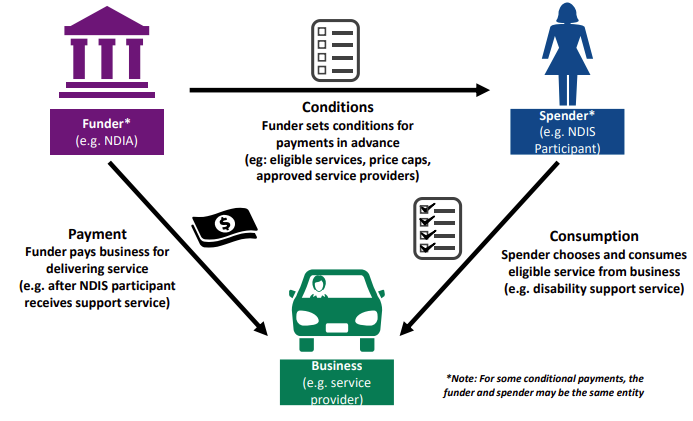
\includegraphics[scale=0.7]{figures/smart_money_network.PNG}  
    \caption{The structure of a smart money network as outlined by Royal et al.\cite{royal}}
    \label{fig:my_label}
\end{figure}
The policies attached to the tokens can test all kinds of conditions including the store/service the token is spent at. What kind of goods, how much is spent, and everything that can be written in technical code is an option. The most common aspects that arise should be modeled on the blockchain e.g. type of business, type of purchase, licenses, etc. The possibility to use off-chain data also exists.\\
Smart Sponsor takes inspiration from this original design by Royal et al.\cite{royal}. However, it puts more of a focus on proving attached conditions. Whereas Weber "burns" the tokens after use and treats them as food stamps \cite{weber}\cite{pattern}, Smart Sponsor will allow these tokens to be used and reused, acting only temporarily as vouchers.